\subsection{Grobkonzept 2} \label{subsec:grobkonzept2}
\begin{table}[H]
\footnotesize
\begin{tabular}{>{\HY\RaggedRight}p{3cm} >{\HY\RaggedRight}p{2.2cm} >{\HY\RaggedRight}p{4cm} >{\HY\RaggedRight}p{3.3cm} >{\HY\RaggedRight}p{1.2cm}}
\hline
	\textbf{Bestandteil}		&\textbf{Typ}			&\textbf{Funktion}									&\textbf{Specs}			&\textbf{Anz.}\\
\hline
\rowcolor{dgelb}
\multicolumn{5}{l}{\textbf{Stromerzeugung}}\\
	Turbine 					&Pelton 				&Umwandlung in Rotationsenergie						&							&1	\\
	Generator					&Gleichstrom 			&Umwandlung in elektrische Energie					&	 						&1	\\
\rowcolor{dblau}
\multicolumn{5}{l}{\textbf{Elektrotechnik}}\\
 	Wechselrichter				&						&Einspeisung ins Stromnetz							&							&1	\\
 	Zentrale Ventilsteuerung	&						&Öffnet/schliesst Ventile je nach Füllstand			&							&1	\\
\rowcolor{dpink}
\multicolumn{5}{l}{\textbf{Bedienung}}\\
 	Anzeige 					&LCD-Display			&zeigt Tankfüllstände und die Generatordaten an 	&							&1	\\
 	Warnsystem					&						&Warnt bei zu hochem Füllstand in einem der Tanks 	&							&1	\\
\rowcolor{dgruen}
\multicolumn{5}{l}{\textbf{Abwassertechnik}}\\
	Tanks 						& 						&Zwischenspeicher für Abwasser 						&4m3, trichterförmig		&5 	\\
	Ablassventil				&						&Entlässt das Abwasser aus dem Tank 				&							&5	\\
	Entlüftung					&						&Ermöglicht Luftaustausch, entlässt Gase			&							&5	\\
	Notüberlauf					&						&Verhindert, dass Tank zu voll wird					&							&5	\\
	Füllstandsensor				&Ultraschall			&Misst den Füllstand des Tanks						&Messbereich <20cm bis >3m	&5	\\
	Druckleitungen				&						&Machen hohe Wassersäulen möglich?					&Druckfestigkeit >40 bar	&5	\\
	Bypass für Turbine 			&Manuell				&Ermöglicht Wartung der Turbine 					&							&1	\\
	Bypass für Tanks 			&Manuell				&Ermöglicht Wartung und Reingung der Tanks 			&	 						&5	\\
	Einwegventile				&						&Verhindern Rückfluss 								&							&4	\\
\hline
\end{tabular}
\end{table}
\newpage
\begin{wrapfigure}{r}{0.5\textwidth}
  \begin{center}
    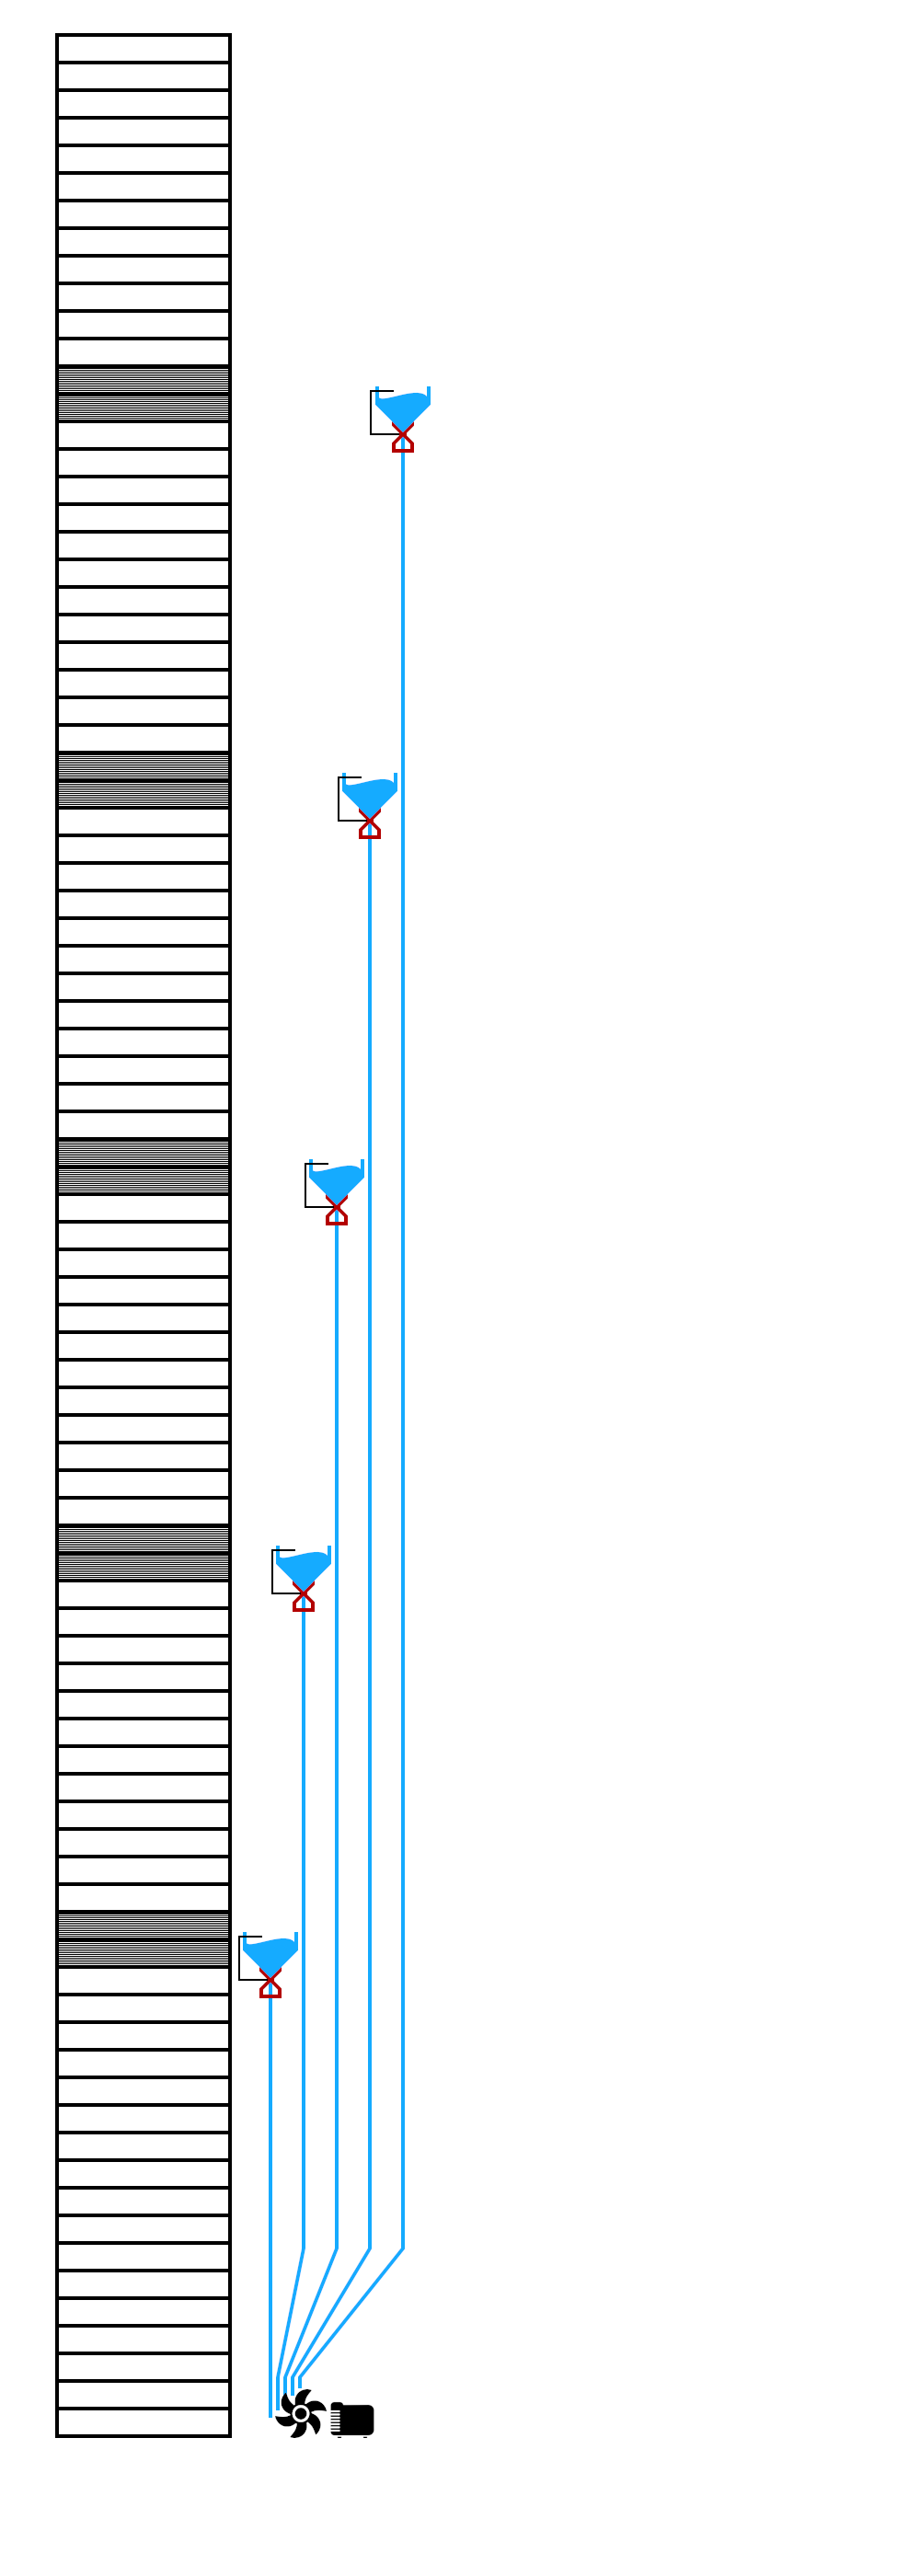
\includegraphics[width=0.48\textwidth]{grobkonzept2}
  \end{center}
  \caption{Grobkonzept 2}
\end{wrapfigure}
Im Grobkonzept 2 soll die Energieausbeutung gesteigert werden, indem das Abwasser zuerst in Tanks gespeichert wird, die all 14 Stockwerke eingebaut sind. In unserem Hochmausmodell an der Park Avenue 432 in New York gibt es all 14 Stockwerke zwei Zwischenstockwerke, wo der Einbau möglich wäre. Wenn der Füllstandsensor im Tank erkennt, dass er voll ist, wird ein Ventil geöffnet und das Wasser fliesst durch eine Druckleitung in den Keller, wo es eine Pelton-Turbine mit Generator antreibt. Die gewonnene Elektrische Energie wird über einen Wechselrichter dem Stromnetz zugeführt. Auf diese Art und Weise braucht man auch nur eine Turbine, die von mehreren Tanks gespeist werden kann.\\ 
Da das Abwasser das Rohr komplett ausfüllt, gibt es keinen Luftwiderstand, der es abbremst. So kann der Wirkungsgrad des Systems verbessert werden. Nur für eine Kurze zeit, bis das Rohr komplett mit Wasser gefüllt ist, tritt Luftwiderstand auf.\\
Da es im Modellhochhaus in den letzten 17 Stockwerken kein Zwischenstockwerk mehr gibt, bleibt das Abwasser dieser Stockwerke ungenutzt.\\
Die baulichen Massnahmen, die nötig sind, um dieses System zu installieren sind beträchtlich. Es müssen Tanks eingebaut werden, Druckleitungen zur Turbine verlegt werden, die im Keller installiert werden muss, und die bestehenden Abwasserleitungen anders verlegt werden, dass sie in die Tanks führen. Somit ist es eher für Neubauten geeignet als zur Nachrüstung.\\

\subsubsection{Wartung}
Um zu verhindern, dass es in den Tanks zu Ablagerungen kommt, ist der Boden der Tanks trichterförmig. So werden alle Ablagerungen beim Öffnen des Ventils weggespült. Sollte es doch nötig sein, die Tanks zu Reinigen, gibt es ein Bypass mit dem das Abwasser an einem Tank vorbeigeführt werden kann.\WFclear
Er kann dass entleert und gereinigt oder repariert werden. Auch die Turbine hat einen Bypass, der Wartungsarbeiten ermöglicht.

\subsubsection{Sicherheitsmassnamen}
Jeder Tank ist mit einem Überlauf ausgestattet, der Verhindert, dass ein Tank zu voll wird wenn z.B. der Ablauf verstopft ist. Das überschüssige Abwasser wird dann in einem Rohr in die Fallleitung Stockwerke tiefer geleitet. Von dort gelangt es dann in den nächsten Abwassertank. Der Füllstandsensor im Tank erkennt, wenn der Pegel zu hoch wird und sendet eine Warnung.
Falls aus irgendeinem Grund mehr als eines der Ventile gleichzeitig geöffnet würde, könnte es zu einem Rückstau kommen, bei dem Abwasser durch die Druckleitungen von dem höher gelegenen Tank in einen tieferen fliesst. Um dies zu verhindern,werden in den Druckleitungen Einwegventile eingebaut. Der höchstgelegene Tank benötigt kein solches Ventil. 


\textbf{Vorteile:} 									\newline
+	Kein Luftwiderstand (sobald Rohr gefüllt ist)	\newline
+	Nur eine Turbine nötig							\newline

\textbf{Nachteile:}									\newline
-	Braucht viel Platz 								\newline
-	Grössere Bauliche Massnahmen nötig				\newline
-	Verstopfungsgefahr 								\newline
-	Lange Leitungen brauchen länger bis komplett mit Wasser gefüllt, bis dann Luftwiderstand
-	das Abwasser der letzten 17 Stockwerke bleibt ungenutzt